\documentclass[titlepage]{article}
\usepackage{graphicx}
\graphicspath{{img/}}
\usepackage[spanish]{babel}
\usepackage{float}

\title{Proyecto: Shell}
\author{Hector Manuel Larios Ponce y Gabriel Patricio Balam Flores}
\date{22/09/2023}

\begin{document}

\maketitle
\tableofcontents
\pagebreak

%============================================================================
\section{Introducción}
El proyecto consiste en desarrollar un programa que simule una terminal de trabajo con shell script. En esta terminal se podrá trabajar a través de línea de comandos que aceptará ciertas palabras para la ejecución de scrips. Estos comandos permiten consultar la información del sistema, reproducir música, ver hora y fecha, buscar archivos y jugar minijuegos.
\\
\begin{itemize}
\item Inicio de sesión: cuando se corra el programa saltará a la vista un sistema de inicio de sesión simple que detecta los usuarios ya existentes en el sistema operativo y permite el acceso a la terminal. 

\item La prompt: una vez dentro del programa se mostrará una prompt la cual muestra el nombre de usuario, el hostname y la hora. En algunos comandos se agregará a la prompt una nueva sección para mostrar la entrada que se espera.

\item Comandos: cuando se muestre la prompt significa que puedes escribir comandos o en su defecto lo que se te pida.

\item El script fue modificado para que no se permita la salida al programa con el conjunto de teclas CTRL + C y CTRL + Z. Para salir de la terminal existe el comando "salir" que te permitirá la salida del programa.

\end{itemize}

%============================================================================
\newpage
\section{Desarrollo}

Para correr el programa se deberá ejecutar el archivo main.sh con el siguiente comando:
\begin{verbatim}
    ./main.sh
\end{verbatim}

Descripción general de los comandos:
\begin{itemize}
\item \textbf{ayuda}: muestra una lista de los comandos disponibles y una breve descripción de su funcionamiento.                        
\item \textbf{feho}: muestra la hora y fecha actual.
\item \textbf{creditos}: despliega los créditos de todo el código. 
\item \textbf{search}: busca un archivo especificado en la ubicación dada. 
\item \textbf{infosys}: muestra los datos técnicos del sistema operativo de hardware. 
\item \textbf{game}: permite al usuario interactuar con diferentes juegos de terminal preestablecidos.               
\item \textbf{bashmusic}: abre un reproductor de música con interfaz gráfica.           
\item \textbf{exit}: termina la ejecución del programa.     
\item \textbf{clear}: limpia la pantalla. 
\end{itemize}

%============================================================================
\newpage
\section{Desarrollo: descripción de los comandos.}

% AYUDA -----------------------------------------------
\noindent
\textbf{Comando:} \verb|ayuda|. \\
\textbf{Descripción:} muestra una tabla de los comandos disponibles y una breve descripción de su funcionamiento.

\begin{figure}[H]
    \centering
    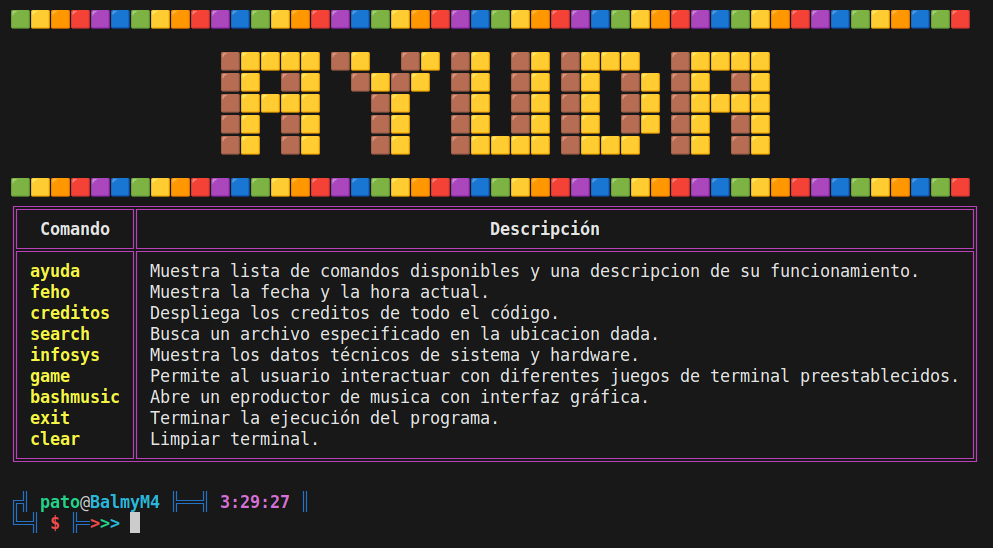
\includegraphics[width=0.8\textwidth]{ayuda.png}
    \caption{Ejecución del comando \textbf{ayuda}:}
    \label{fig:ejemplo}
\end{figure}

% FEH0 -----------------------------------------------
\noindent
\textbf{Comando:} \verb|ayuda|. \\
\textbf{Descripción:} acrónimo de fecha y hora, el comando muestra la hora y fecha actual. Esta información se obtiene del archivo /proc/driver/rtc, el cual contiene información sobre el real time clock del sistema. Su funcionamiento consiste en identificar los datos rtc time y rtc date en el archivo con el comando grep, para posteriormente guardar los datos con awk en una variable local.

\begin{figure}[H]
    \centering
    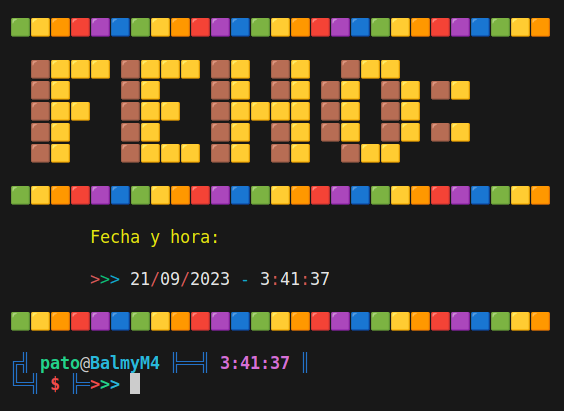
\includegraphics[width=0.7\textwidth]{feho.png}
    \caption{Ejecución del comando \textbf{feho}:}
    \label{fig:ejemplo}
\end{figure}

% creditos -----------------------------------------------
\noindent
\textbf{Comando:} \verb|creditos|. \\
\textbf{Descripción:} despliega una tabla que contiene los créditos del código.

\begin{figure}[H]
    \centering
    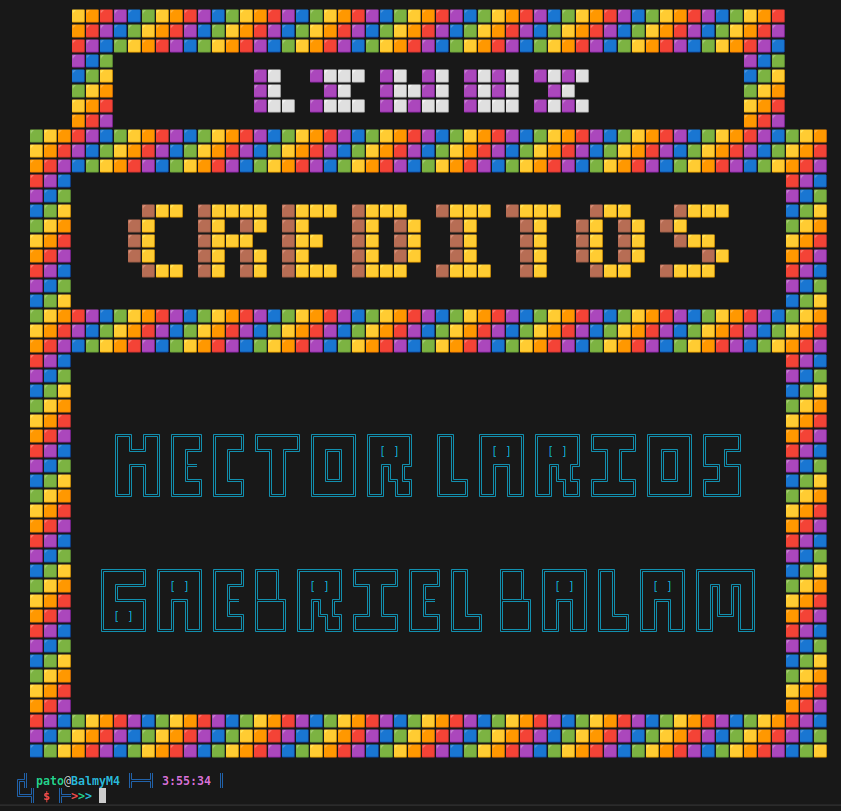
\includegraphics[width=0.75\textwidth]{creditos.png}
    \caption{Ejecución del comando \textbf{creditos}:}
    \label{fig:ejemplo}
\end{figure}

% search -----------------------------------------------
\noindent
\textbf{Comando:} \verb|search|. \\
\textbf{Descripción:} al escribir el comando te redirige a un apartado donde se te piden dos parámetros, el nombre del archivo a buscar y la ruta donde se va a buscar. Si la ruta dada no es absoluta, el programa lo detecta y cambia a un modo automático de ruta relativa partiendo de HOME.

\begin{figure}[H]
    \centering
    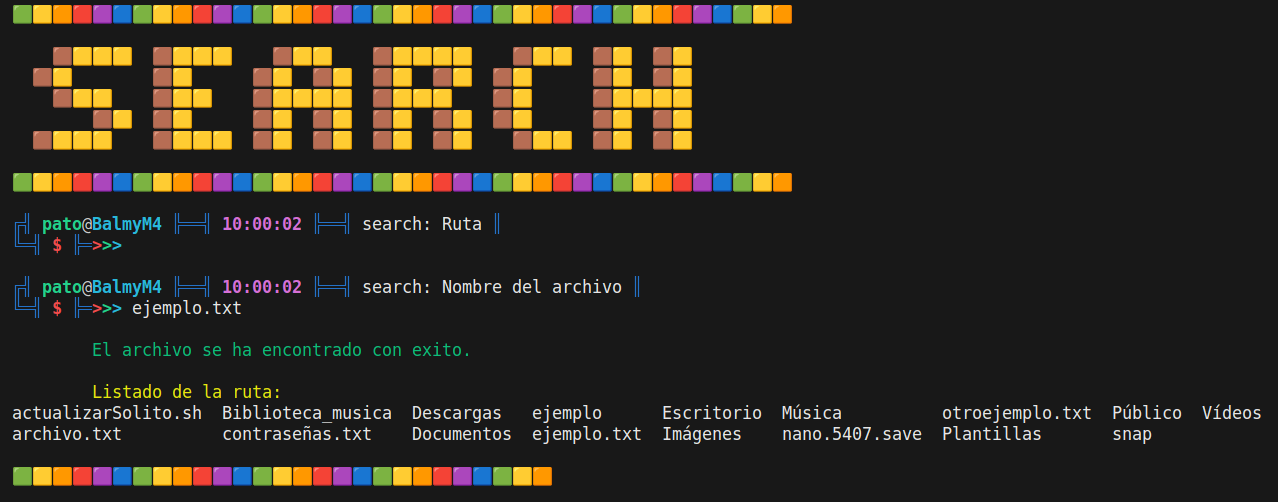
\includegraphics[width=0.9\textwidth]{search.png}
    \caption{Ejecución del comando \textbf{search}:}
    \label{fig:ejemplo}
\end{figure}

% infosys -----------------------------------------------
\noindent
\textbf{Comando:} \verb|infosys|. \\
\textbf{Descripción:} muestra algunos datos técnicos del sistema operativo y de hardware. En la figura 5 se observan todos los datos que muestra el comando.

\begin{figure}[H]
    \centering
    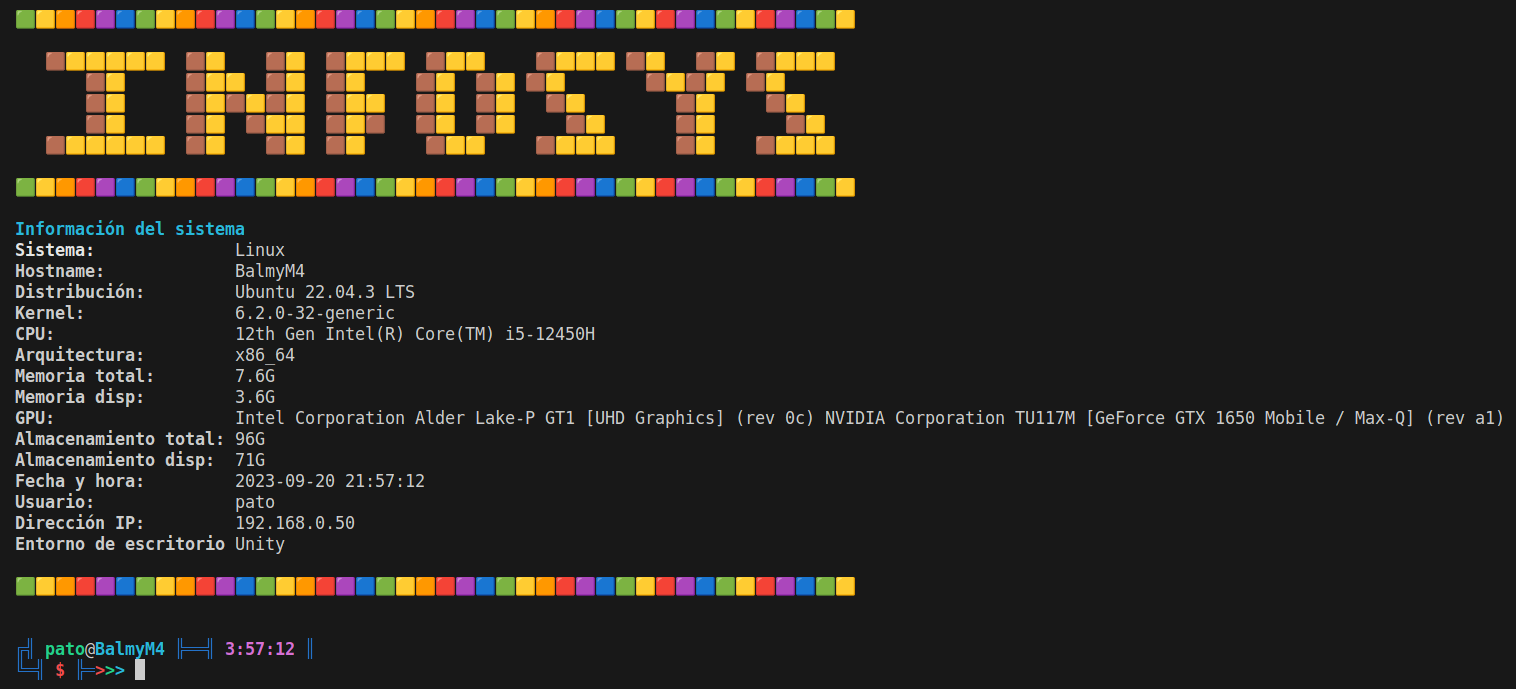
\includegraphics[width=0.8\textwidth]{infosys.png}
    \caption{Ejecución del comando \textbf{infosys}:}
    \label{fig:ejemplo}
\end{figure}

% game -----------------------------------------------
\noindent
\textbf{Comando:} \verb|game|. \\
\textbf{Descripción:} al ejecutar el comando se redirige a un apartado de selección de minijuegos. Hay tres minijuegos disponibles, el segundo es el típico piedra papel o tijeras en el cual se escogerá aleatoriamente la opción del oponente. El primer minijuego consiste en adivinar un número seleccionado aleatoriamente a través de pistas que se te irán dando. El último minijuego consiste en resolver cinco laberintos disponibles. 

\begin{figure}[H]
    \centering
    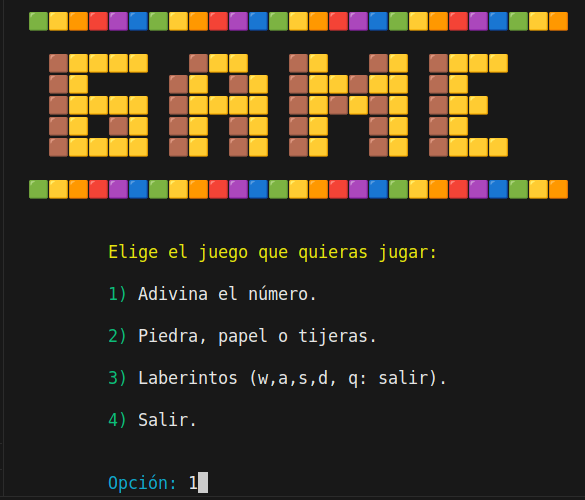
\includegraphics[width=0.7\textwidth]{game.png}
    \caption{Ejecución del comando \textbf{game}:}
    \label{fig:ejemplo}
\end{figure}

% bashmusic -----------------------------------------------
\noindent
\textbf{Comando:} \verb|bashmusic|. \\
\textbf{Descripción:} abre un reproductor de música con interfaz gráfica.          

\begin{figure}[H]
    \centering
    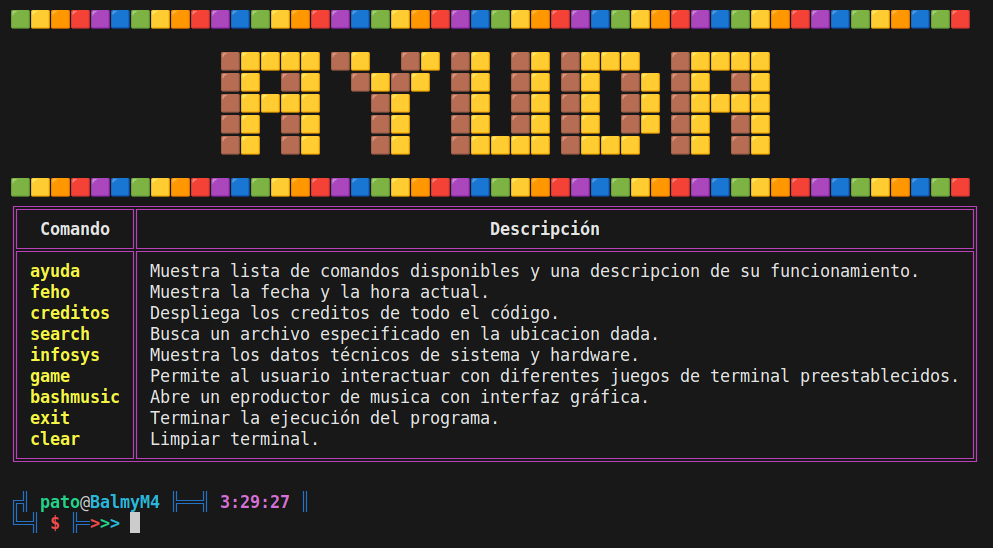
\includegraphics[width=0.9\textwidth]{ayuda.png}
    \caption{Ejecución del comando \textbf{bashmusic}:}
    \label{fig:ejemplo}
\end{figure}

% exit -----------------------------------------------
\noindent
\textbf{Comando:} \verb|exit|. \\
\textbf{Descripción:} termina la ejecución del programa.           

\begin{figure}[H]
    \centering
    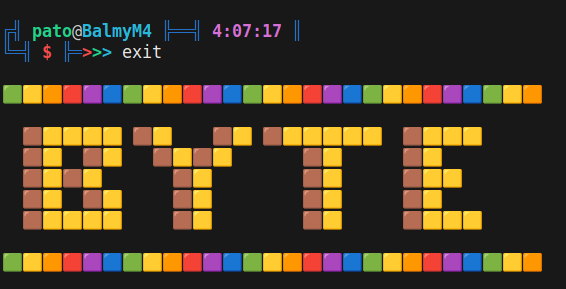
\includegraphics[width=0.9\textwidth]{exit.png}
    \caption{Ejecución del comando \textbf{exit}:}
    \label{fig:ejemplo}
\end{figure}
 

%============================================================================
\newpage
\section{Conclusiones}
\textbf{Hector Manuel Larios Ponce}:\\
\\\\

\textbf{Gabriel Patricio Balam Flores}:\\


\end{document}
